\documentclass[letterpaper]{sae}
\usepackage{graphicx}
\usepackage{mathptmx}
\usepackage{float}
\usepackage[cmex10]{amsmath}
\usepackage{amsthm,amssymb}
\usepackage{url}
\urlstyle{same} 
\def\UrlBreaks{\do\/\do-}
\usepackage{fancybox}
\usepackage{breqn}
\usepackage{array}
\usepackage{caption}
\usepackage{subcaption}
\usepackage{comment}
\usepackage[english]{babel}
\usepackage[acronym,nomain]{glossaries} % list of acronyms
\usepackage{multirow}
\usepackage{tocloft}
\usepackage{multicol}


\newacronym{ghg}{GHG}{Green-House Gas}
\newacronym{fe}{FE}{Fuel Economy}
\newacronym{ee}{EE}{Energy Economy}
\newacronym{epa}{EPA}{Environmental Protection Agency}
\newacronym{oem}{OEM}{Original Equipment Manufacturer}
\newacronym{ice}{ICE}{Internal Combustion Engine}
\newacronym{icv}{ICV}{Internal Combustion Vehicle}
\newacronym{icev}{ICEV}{Internal Combustion Engine Vehicle}
\newacronym{em}{EM}{Electric Motor}
\newacronym{hev}{HEV}{Hybrid Electric Vehicle}
\newacronym{ev}{EV}{Electric Vehicle}
\newacronym{phev}{PHEV}{Plug-in Hybrid Electric Vehicle}
\newacronym{lrphev}{LR-PHEV}{Long Range PHEV}
\newacronym{srphev}{SR-PHEV}{Short Range PHEV}
\newacronym{mhev}{MHEV}{Mild Hybrid Electric Vehicle}
\newacronym{pev}{PEV}{Plug-in Electric Vehicle}
\newacronym{bev}{BEV}{Battery Electric Vehicle}
\newacronym{cbev}{CBEV}{City BEV}
\newacronym{afv}{AFV}{Alternative Fuel Vehicle}
\newacronym{fcev}{FCEV}{Fuel Cell Electric Vehicle}
\newacronym{cav}{CAV}{Connected Autonomous Vehicle}
\newacronym{fc}{FC}{Fuel Consumption}
\newacronym{ec}{EC}{Energy Consumption}
\newacronym{dtto}{DTTO}{Discrete Time Trajectory Optimization}
\newacronym{udto}{UDTO}{Uniformly Discretized Trajectory Optimization}
\newacronym{sto}{STO}{Spline Trajectory Optimization}
\newacronym{rbed}{RBED}{Rules-Based Eco-Driving}
\newacronym{cidm}{CIDM}{Cooperative Intelligent Driver Model}
\newacronym{idm}{IDM}{Intelligent Driver Model}
\newacronym{soc}{SOC}{State of Charge}
\newacronym{ocp}{OCP}{Optimal Control Problem}
\newacronym{ttc}{TTC}{Time-To-Collision}
\newacronym{dp}{DP}{Dynamic Programming}
\newacronym{ga}{GA}{Genetic Algorithm}
\newacronym{sdm}{SDM}{Smart Driver Model}
\newacronym{v2i}{V2I}{Vehicle to Infrastructure}
\newacronym{v2v}{V2V}{Vehicle to Vehicle}
\newacronym{v2x}{V2X}{Vehicle to Everything}
\newacronym{hil}{HIL}{Hardware In Loop}
\newacronym{pso}{PSO}{Particle Swarm Optimization}
\newacronym{dt}{DT}{Direct Transcription}
\newacronym{oedt}{OEDT}{Optimal Eco-Driving Trace}
\newacronym{fods}{FODS}{Forward Object Detection System}
\newacronym{cas}{CAS}{Collision Aviodance System}
\newacronym{acc}{ACC}{Adaptive Cruise Control}
\newacronym{obu}{OBU}{On-Board Unit}
\newacronym{rsu}{RSU}{Road-Side Unit}
\newacronym{sae}{SAE}{Society of Automotive Engineers}
\newacronym{adas}{ADAS}{Advanced Driver Assistance System}
\newacronym{edc}{EDC}{Eco-Driving Control}
\newacronym{lv}{LV}{Lead Vehicle}
\newacronym{ss}{SS}{Segment Speeds}
\newacronym{hs}{HS}{Historical Speeds}
\newacronym{spat}{SPAT}{Signal Phase and Timing}
\newacronym{map}{MAP}{Positions of Subsequent Traffic Lights}
\newacronym{al2n}{AL2N}{Acceleration L\textsuperscript{2} Norm}
\newacronym{rpc}{RPC}{Road Power Cost}
\newacronym{bpc}{BPC}{Battery Power Cost}
\newacronym{fecc}{FECC}{Fitted Equivalent Consumption Cost}
\newacronym{ipopt}{IPOPT}{Interior-Point Optimization}
\newacronym{dtnlp}{DTNLP}{Discreet-Time Non-Linear Programming}
\newacronym{snlp}{SNLP}{Spline Non-Linear Programming}
\newacronym{sga}{SGA}{Spline Genetic Algorithm}
\newacronym{spso}{SPSO}{Spline Particle Swarm Optimization}
\newacronym{2sdp}{2SDP}{2 State Dynamic Programming}
\newacronym{aos}{AOS}{Approximate Optimal Spline}
\newacronym{pchip}{PCHIP}{Piecewise Cubic Hermitic Interpolation Polynomial}
\newacronym{nrel}{NREL}{National Renewable Energy Laboratory}
\newacronym{fastsim}{FASTSim}{Future Automotive Systems Technology Simulator}
\newacronym{mfei}{MFEI}{Mean Fuel Economy Improvement}
\newacronym{pas}{PAS}{Percent Acceptable Solutions}
\newacronym{mrt}{MRT}{Mean Run-Time}
\newacronym{mpc}{MPC}{Model Predictive Control}
\newacronym{adp}{ADP}{Approximate Dynamic Programming}
\newacronym{rl}{RL}{Reinforcement Learning}
\newacronym{mbrl}{MBRL}{Model Based Reinforcement Learning}
\newacronym{nlp}{NLP}{Non-Linear Programming}
\newacronym{nhtsa}{NHTSA}{National Highway Traffic Safety Administration}
\newacronym{aeb}{AEB}{Automatic Emergency Braking}
\newacronym{tsdc}{TSDC}{Transportation Secure Data Center}
\newacronym{anl}{ANL}{Argonne National Lab}
\newacronym{d3}{D\textsuperscript{3}}{Downloadable Dynamometer Database}
\newacronym{cd}{C\textsubscript{D}}{Coefficient of Drag}
\newacronym{crr}{C\textsubscript{RR}}{Coefficient of Rolling Resistance}
\newacronym{mape}{MAPE}{Mean Absolute Percentage Error}
\newacronym{evse}{EVSE}{Electric Vehicle Support Infrastructure}
\newacronym{ld}{LD}{Light Duty}
\newacronym{md}{MD}{Medium Duty}
\newacronym{hd}{HD}{Heavy Duty}
\newacronym{mdhd}{MD/HD}{Medium Duty / Heavy Duty}
\newacronym{inrix}{INRIX}{}
\newacronym{epri}{EPRI}{Electric Power Research Institute}
\newacronym{nhts}{NHTS}{National Highway Transportation Survey}
\newacronym{usa}{USA}{United States of America}
\newacronym{sof}{SOF}{State of Fuel}
\newacronym{hc}{HC}{Home Charging}
\newacronym{bc}{BC}{Battery Capacity}
\newacronym{dcl}{DCL}{Destination Charger Likelihood}
\newacronym{ercr}{ERCR}{En-Route Charging Rate}
\newacronym{ercp}{ERCP}{En-Route Charging Penalty}
\newacronym{ftc}{FTC}{Fuel Tank Capacity}
\newacronym{ftp}{FTP}{Fuling Time Penalty}
\newacronym{psrc}{PSRC}{Puget Sound Regional Council}
\newacronym{bts}{BTS}{Bureau of Transportation Statistics}
\newacronym{happ}{HAPP}{Household Activity Pattern Problem}
\newacronym{chts}{CHTS}{California Houslehold Travel Survey}
\newacronym{dcfc}{DCFC}{DC Fast Charging}
\newacronym{liion}{Li-Ion}{Lithium-Ion}
\newacronym{lvl2}{LVL 2}{DC Level 2}
\newacronym{oems}{OEMS}{Optimal Energy Management Strategies}
\newacronym{poems}{POEMS}{Predictive Optimal Energy Management Strategies}
\newacronym{vpoems}{VP-OEMS}{Velocity Prediction enabled Optimal Energy Management Strategies}
\newacronym{gnss}{GNSS}{Global Navigational Satellite System}
\newacronym{obd2}{OBD-II}{On-Board Diagnostics II}
\newacronym{csu}{CSU}{Colorado State University}
\newacronym{wes}{WES}{Weight Efficiency Score}
\newacronym{gvwr}{GVWR}{Gross Vehicle Weight Rating}
\newacronym{fha}{FHA}{Federal Highway Administration}
\newacronym{vius}{VIUS}{Vehicle Inventory and Use Survey}
\newacronym{eod}{EOD}{End of Day}
\newacronym{osrm}{OSRM}{Open-Source Routing Machine}
\newacronym{vrp}{VRP}{Vehicle Routing Problem}
\newacronym{evrp}{EVRP}{Electric Vehicle Routing Problem}
\newacronym{tsp}{TSP}{Traveling Salesman Problem}
\newacronym{can}{CAN}{Controller Area Network}
\newacronym{lstm}{LSTM}{Long Short-Term Memory}
\newacronym{ann}{ANN}{Artificial Neural Network}
\newacronym{ml}{ML}{Machine Learning}
\newacronym{fcdp}{FC-DP}{Full Cycle Dynamic Programming}
\newacronym{ppmpc}{PP-MPC}{Perfect Prediction Model Predictive Control}
\newacronym{rpmpc}{RP-MPC}{Real Prediction Model Predictive Control}
\newacronym{cvmpc}{CV-MPC}{Constant Velocity Model Predictive Control}
\newacronym{mae}{MAE}{Mean Absolute Error}
\newacronym{fsmvrp}{FSMVRP}{Fleet Size and Mix Vehicle Routing Problem}
\newacronym{mcvrp}{MCVRP}{Monte-Carlo Vehicle Routing Problem}
\newacronym{ppf}{PPF}{Percent Point Function}
\newacronym{ccdng}{CCDNG}{Completely Connected Directional Network Graph}
\newacronym{sho}{SHO}{Spline Heuristic-Optimal}
\newacronym{npv}{NPV}{Net Present Value}
\newacronym{tco}{TCO}{Total Cost of Ownership}
\newacronym{mtk}{MTK}{Metric-Ton-Kilometer}
\newacronym{lco}{LCO}{Levelized Cost of Ownership}
\newacronym{lcod}{LCOD}{Levelized Cost of Driving}
\newacronym{sme}{SME}{Subject Matter Expert}
\newacronym{doe}{DOE}{Deparment of Energy}
\newacronym{vmt}{VMT}{Vehicle Miles Traveled}
\newacronym{dot}{DOT}{Department of Transportation}
\newacronym{ltl}{LTL}{Less Than Truckload}
\newacronym{lpcp}{LPCP}{Lost Payload Capacity Portion}
\newacronym{chaas}{ChaaS}{Charging as a Service}
\newacronym{tou}{TOU}{Time of Use}
\newacronym{ocs}{OCS}{Optimal Charging Strategy}
\newacronym{soe}{SOE}{State of Energy}
\newacronym{ltp}{LTP}{Lost Time Portion}
\newacronym{yd}{YD}{Yearly Distance}
\newacronym{dd}{DD}{Daily Distance}
\newacronym{vnr}{VNR}{Vehicle Nominal Range}
\newacronym{nyo}{NYO}{Number of Years of Ownership}
\newacronym{ap}{AP}{Age at Purchase}
\newacronym{dpm}{DPM}{Diesel Price Multiplier}
\newacronym{epm}{EPM}{Electricity Price Multiplier}
\newacronym{evsep}{EVSEP}{EVSE Premium}
\newacronym{pe}{PE}{Payload Exemption}
\newacronym{bpp}{BPP}{Battery Pack Pricing}
\newacronym{my}{MY}{Model Year}
\newacronym{ipfn}{IPFN}{Iterative Proportional Fitting with N dimensions}
\newacronym{dco}{DCO}{Discretized Control Optimization}
\newacronym{pto}{PTO}{Polynomial Trajectory Optimization}
\newacronym{slsqp}{SLSQP}{Sequential Least Squares Programming}
\newacronym{aer}{AER}{All Electric Range}
\newacronym{msrp}{MSRP}{Manufacturer Recommended Sales Price}
\newacronym{afdc}{AFDC}{Alternative Fuels Data Center}
\newacronym{uf}{UF}{Utility Factor}
\newacronym{hov}{HOV}{Hich Occupancy Vehicle}
\newacronym{lp}{LP}{Linear Problem}
\newacronym{qp}{QP}{Quadratic Problem}
\newacronym{sp}{SP}{Stochastic Problem}
\newacronym{slp}{S-LP}{Stochastic Linear Problem}
\newacronym{milp}{MILP}{Mixed Integer Linear Problem}
\newacronym{smilp}{S-MILP}{Stochastic Mixed Integer Linear Problem}
\newacronym{evcsp}{EVCSP}{Electric Vehicle Charge Scheduling Problem}
\newacronym{sevcsp}{S-EVCSP}{Stochastic Electric Vehicle Charge Scheduling Problem}
\newacronym{phevcsp}{EVCSP}{Plug-in Hybrid Electric Vehicle Charge Scheduling Problem}

\makeglossaries

\raggedbottom
\sloppy

\newcolumntype{C}[1]{>{\centering\let\newline\\\arraybackslash\hspace{0pt}}m{#1-2\tabcolsep}}
\renewcommand{\arraystretch}{1.2}

\PaperTitle{Quantifying the Costs of Charger Availability Uncertainty for Residents of Multi-Unit Dwellings}
\AddAuthor{Author}{Affiliation}
\PaperNumber{2024-XX-XXXX}
\SAECopyright{2024}



\begin{document}
	
\maketitle

\section{abstract}\label{sec:abstract}

Even when charging at the highest rates currently available, \glspl{ev} add range at substantially lower rates than \glspl{icev} do while fueling. In addition, DC charging comes at a cost premium and leads to accelerated battery degradation. EV users able to rely on AC charging during long dwells at home or work may experience cost and time savings relative to \gls{icev} users with similar driving patterns. However, EV users unable to charge during long dwells will face higher charging costs and higher dedicated charging time. An important question is how occupants of \glspl{mud}, which provide some AC \gls{evse} but not enough for all cars to charge at once, will be effected. In this paper the authors’ previously published method for quantifying EV user inconvenience due to charging is extended to deal with stochastic charger availability. \gls{smilp} is used to determine optimal charging behavior for EV users based on itineraries and the likelihood of availability of charging. Expected inconveniences for levels of charger availability and the quantitative value of additional \gls{evse} and of charger scheduling schemes are presented.

\section{Introduction}\label{sec:introduction}

Mass \gls{bev} adoption is a necessary, but not independently sufficient \cite{Iaconangelo_2020,Milovanoff_2020}, step towards meeting transportation de-carbonization goals set out by the US and EU \cite{whitehouse_2021,european_commission_2020}. Currently, \gls{bev} adoption is increasing year-over-year, indicating the success of present policy. Present policy levers utilized by governments to push \gls{bev} purchases largely consist of subsidies which span from direct and indirect purchase incentives to grants for \gls{evse} installation. These subsidies help to overcome the manifest cost and operational disadvantages inherent to \glspl{bev} when compared to \glspl{icev}. Subsidies are justified under the theory that mass adoption will bring economies of scale and negate these disadvantages before the subsidy programs become financially infeasible. There is considerable evidence to support this approach. Increased investment in \gls{bev} production, and particularly \gls{ev} battery production in the previous decade, has resulted in substantial reductions in prices \cite{Sakti_2017}. These are expected continue to a lesser degree in the coming decade \cite{Hsieh_2019} allowing \glspl{bev} to approach cost parity with equivalent \glspl{icev} \cite{Burnham_2021}. Simultaneously, the numbers of private and public \gls{evse} operating in the US have grown tremendously in recent years \cite{AFDC_EVSE_2023} which has somewhat mitigated the operational disadvantages faced by \glspl{bev} for long trips.

Although adoption numbers indicate successful policies to date, there is reason to question the long-term viability of these policies. Current \gls{bev} purchasers and lessees still fit within the paradigm of technological early adopters. Current \gls{bev} adopters are generally older, wealthier, male-skewed, highly educated, and hold positive views of technology \cite{Axsen_2016,Long_2022,Lane_2018,Taherdoost_2018,Straub_2009} when compared to the general population. \glspl{bev} appear most commonly in larger, single-family, suburban households with larger vehicle fleets \cite{MacArthur_2018,ICCT_2022,Fevang_2021,Chakraborty_2022}. The demographics most likely to adopt \glspl{bev} to date are those most able to deal with the pitfalls of \glspl{bev} and most able to utilize the incentives provided. The most effective incentives for driving \gls{bev} adoption have been direct purchase subsidies \cite{Wang_2017,Hardman_2017,Johnson_2017,Roberson_2022,Bjerkan_2016,Diamond_2009} and access subsidies such as use of carpool lanes and preferential parking \cite{Hardman_2019,Chakraborty_2020,Huang_2018,Liu_2021}. Direct purchase subsidies are often reserved for purchasers of new cars and will become unsustainable with high adoption. Access subsidies will become meaningless with high adoption due to saturation effects. While the fundamentals of \gls{bev} use are a disadvantage incentives can only distort the market.

Enthusiastic early adoption does not guarantee eventual mass adoption and, often, new policy approaches are required to continue the trend. \gls{bev} sales have increased year-over-year in recent years but there has also been notable discontinuance. Surveys conducted between 2015 and 2019 on California \gls{ev} buyers who applied for a California Clean Vehicle Rebate showed a discontinuance rate of roughly 18\% for \glspl{bev} \cite{Hardman_2021}. Significant factors leading to discontinuance were dissatisfaction with reliability, range, and charging experience. The availability of AC Level 2 charging at home is critical in determining \gls{bev} charging experience \cite{Lee_2020,Hardman_2018}. The importance of home charging is due to clear and present public \gls{evse} reliability and availability issues \cite{Karanam_2023,Liu_2023,David_2017} which require costly solutions \cite{Gamage_2023,Tal_2022} as well as the inherent convenience of being able to "plug-in and ignore" at home. Modeling efforts suggest that the availability of home charging may lead to a ten-fold decrease in expected dedicated charging time for otherwise identical \gls{bev} users \cite{rabinowitz_IEEE_Access_2023,Dixon_2020}. Home AC level 2 is considerably more likely to be available for residents of \glspl{sud} than residents of \glspl{mud} \cite{Yanbo_2021}, with a similar disparity existing between home owners and renters. A common situation for residents of \glspl{mud} is that the parking lot will have some chargers installed but this number will not be nearly equal to the total number of parking spaces. Thus, residents of \glspl{mud} are left in a situation wherein sufficient charging for all residents may be available but with uncertainty on when said charging will be available for any individual resident.

A critical question is what is required in order to address the \gls{sud}/\gls{mud} disparity. Matching the volume of AC Level 2 \gls{evse} with the volume of \glspl{bev} in \gls{mud} parking lots is an un-economical solution. Travel behavior dynamics dictate that demand will be temporally clustered at any given location. Providing sufficient capacity to match peak demand will require very high costs to be passed on to customers for profitable operation. The objective of \gls{evse} installation incentives is to allocate \gls{evse} resources in order to minimize \gls{bev} user inconvenience subject to constraints on resources. This objective requires not merely comparing supply to demand but understanding how the supply/demand relationship effects user experience.

The central question in this study is what effect uncertainty of charger availability will have on \gls{bev} user experience. Long dwell charging is fundamental to \gls{bev} user behavior due to the relatively slow charging speeds of \glspl{bev} \cite{AFDC_EVs_2023}. As a result, users formulate charging plans and routines rather than charging ad-hoc \cite{Bunce_2014,Chakraborty_2019,Dunckley_2016}. Formulating charging plans and routines is a simpler task with better future information. With imperfect future information, rational agents will sacrifice optimality in order to reduce risk, especially if the downside is substantial. For \gls{bev} users, the ultimate downside risk is an extremely inconvenient event such as having insufficient range to complete an intended trip. For drivers engaged in long trips or trip chains, a stranding event can sometimes be triggered by one or several failed charge events \cite{Karanam_2023}. For drivers completing routine travel in a populated environment, the downside is being forced to delay for significant time and/or travel out of the way to charge. Desire to avoid downside risk can lead \gls{bev} drivers to elect for less convenient charge events as part of their regular behavior. By this theory, one would expect that the inconvenience cost of charging a \gls{bev} due to scarce and uncertain charging opportunities will be non-negligibly greater than that which arises from scarce but predictable charging opportunities. In this paper, the value of information associated with charger availability uncertainty is assessed quantitatively and results are presented along with ensuing operational and policy implications.

\section{Methods}\label{sec:methods}

This study serves to test the hypothesis that there is an inconvenience cost-of-uncertainty associated with reliance on public and shared \gls{evse}. This hypothesis is evaluated by comparing how theoretical \gls{bev} users would charge their vehicles with perfect and imperfect information about charger availability in the future. The scope of this analysis is limited to routine commuter travel behavior. Drivers with unpredictable driving routines and/or very high daily travel distances (such as ride-sharing and delivery drivers) or very low daily travel requirements (such as home-workers) will naturally have to rely more on ad-hoc charging. Routine commuter driving constitutes the bulk of light-duty driving \cite{nhts_2017} and is the focus herein. The method of evaluation in this study is to compare the dedicated charging time required for the exact same itineraries with perfect and imperfect future information. This is accomplished via comparing the optimal charging schedules generated for a given itinerary using  \glsunset{milp}\gls{milp} with perfect information and \gls{smilp} with imperfect information. The method relies in the following assumptions:

\begin{description}
	\item [A.1:] Charging a vehicle is only inconvenient for the amount of time that a user has to devote to charging said vehicle.
	\item [A.2:] \gls{bev} users will attempt to schedule charging events in a manner which minimizes inconvenience.
	\item [A.3:] For a given vehicle and itinerary the characteristic inconvenience cost is the minimum inconvenience cost.
\end{description}

A possible shortcoming of this method is that \gls{bev} users may optimize for charging cost as well as charging inconvenience. Some evidence exists that \gls{bev} users will opt to charge away from home if doing so is cheaper \cite{Lee_2020}. However, charging costs are difficult to model and vary considerably due to factors such as charger network, time-of-day, location, incentives, etc. making precise integration of financial charging costs into the optimization imprecise. Furthermore, it is largely true that high-rate charging typical of dedicated charging stations is more expensive on a per-kWh basis than the low-rate charging typical of long-dwell charging at home, work, or retail locations \cite{Trinko_2021}. Thus the type of charge events selected by an inconvenience minimization strategy should be the same as those selected by a financial cost minimization strategy.

\subsection{Metric of Optimization}

In order to assess inconvenience cost-of-uncertainty, a metric of inconvenience must be defined. In this study the Inconvenience Score ($S_{IC}$) metric from \cite{rabinowitz_IEEE_Access_2023} is used. The $S_{IC}$ metric is an implementation of the logic of assumption A.1. $S_{IC}$ defined as

\begin{equation}
	S_{IC}=\frac{\sum_{k=0}^{N}[D_{E,k}M_{E,k}+D_{T,k}M_{T,k}+D_{P,k}M_{P,k}]}{\sum_{k=0}^{N}L_k}\label{eq:sic}
\end{equation}

for an itinerary of $N$ trips where $D_E$ is the duration of the charging event, $D_T$ is the duration of travel to get to the charging location, $D_P$ is the duration of the payment process, $M_{E,k}$, $M_{T,k}$, and $M_{P,k}$ are integer multipliers which respectively define whether or not to count the various durations for trip $k$, and $L_k$ is the length of trip $k$ in kilometers. $S_{IC}$, thus, is the average dedicated charging time per kilometer traveled in a given itinerary. The values of the multipliers based on the type of charging event are shown in Table \ref{tab:met:sic:multipliers}.

\begin{table}[H]
	\centering
	\caption{Values of multipliers based on charging event type}\label{tab:met:sic:multipliers}
	\begin{tabular}{|C{\linewidth/2}|C{\linewidth/6}|C{\linewidth/6}|C{\linewidth/6}|}
		\hline Energizing Event Type & $M_E$ & $M_T$ & $M_P$ \\
		\hline Home & 0 & 0 & 0 \\
		\hline Work & 0 & 0 & 0 \\
		\hline Destination & 0 & 0 & 1 \\
		\hline En-route & 1 & 1 & 1 \\
		\hline
	\end{tabular}
\end{table}

$S_{IC}$ reflects the differences in dedicated time spent by charging event type. Charging events that fit into dwells in an existing itinerary are substantially less inconvenient than those which require alterations to an existing itinerary.

\subsection{Optimization}

The objective of the optimization is to find the charge schedule which minimizes $S_{IC}$ for a given itinerary and given charger availability. As seen in \eqref{eq:sic}, much of $S_{IC}$ accrued during a given charge event arises from the travel and payment penalties. Thus, $S_{IC}$ is discontinuous around zero. In order to make the problem solvable with integer-linear solvers the decision variables are split into Booleans which represent the decision to charge during a given dwell or trip and linear variables which represent the duration of the charge event. Each potential charge event has a known charging rate. This combination of variables allows for the problem to be solved as a \gls{milp}. In order to evaluate the cost-of-uncertainty the problem must be formulated in both a deterministic and a stochastic manner. The deterministic formulation allows for optimization to take place for one defined itinerary with known charger rates and availability and reflects optimization with perfect future knowledge. The stochastic formulation allows for a single optimal solution to be computed considering all scenarios (same itinerary but different charger availabilities) within a set. This is accomplished by separating decision variables into first-stage decision variables which influence all scenarios and second-stage decision variables which influence only the specific scenario. In this case the Booleans are first-stage and the linear variables are second-stage. In other words, the theory is that \gls{bev} users will have to plan when to charge but may alter durations to suit their needs. The stochastic formulation reflects optimization with imperfect future knowledge.

\subsubsection{Deterministic Formulation}

To minimize the number of decision variables, and thus solver run-time, the objective is formulated differently than in \eqref{eq:sic}. For the deterministic optimization the objective function is

\begin{equation}
	\min_{u\in U}\quad \sum_{e\in E}[u_e^{db}c_e^{db}+u_e^{ab}c^{ab}+u_e^{ad}c^{ad}] \label{eq:obj}
\end{equation}

where $E$ is the set of itinerary events (trip then dwell), $U=\{u^{dd},u^{db},u^{ad},u^{ab}\}$ is the set of decision variables including, in order, dwell charge event duration, dwell charge event Boolean, ad-hoc charge event duration, ad-hoc charge event Boolean, and  $C=\{c^{dd},c^{db},c^{ad},c^{ab}\}$ is the set of constant cost multipliers corresponding to $U$. The components of $C$ have values corresponding to the multipliers in \eqref{eq:sic} and Table \ref{tab:met:sic:multipliers}. The cost $c^{dd}$ is assumed to be zero because charge events which occur during planned dwells are assumed to not inconvenience the driver except for the time required to initiate the charge event. Because of this, and in order to reduce the dimensionality of the optimization, the term $u_e^{dd}c^{dd}$ is omitted from \eqref{eq:obj}. The other costs in $C$ are tunable parameters and values used in this paper are $c^{db} = 1$, $c^{ab} = 5$, and $c^{ad} = 1$ all in minutes. The variables in \eqref{eq:obj} are bounded as follows

\begin{equation}
	\begin{array}{ccc}
		\multicolumn{3}{c}{b^{dd,l}u_{e}^{db}-u_{e}^{dd}\leq 0}\\
		\multicolumn{3}{c}{b^{dd,u}u_{e}^{db}-u_{e}^{dd}\geq 0}\\
		\multicolumn{3}{c}{b^{ad,l}u^{ab}-u_{e}^{ad}\leq 0}\\
		\multicolumn{3}{c}{b^{ad,u}u^{ab}-u_{e}^{ad}\geq 0}\\
		& s.t. & \\
		u^{db}, u^{ab}\in\mathbb{B} && \forall e\in E\\
	\end{array}
\end{equation}

where $b = \{b^{ad,1}, b^{ad,u}, b^{dd,l}, b^{dd,u}\}$ is the set of lower and upper bounds for AC and DC charge event durations. The problem is subject to several constraints which serve the purpose of maintaining the vehicle's \gls{soc} within allowed limits and returning the vehicle's \gls{soc} to a given final value. these constraints are

\begin{equation}
	s_i+\sum_{k=0}^{K}[u_{e_k}^{dd}r_{e_k}^{d}+u_{e_k}^{ad}r_{e_k}^{a}-d_{e_k}]\geq s_{l}\quad \forall K\in E
\end{equation}
\begin{equation}
	s_i+\sum_{k=0}^{K}[u_{e_k}^{dd}r_{e_k}^{d}+u_{e_k}^{ad}r_{e_k}^{a}-d_{e_k}]\leq s_{u}\quad \forall K\in E
\end{equation}
\begin{equation}
	s_i+\sum_{e\in E}[u_{e}^{dd}r_{e}^{d}+u_{e}^{ad}r_{e}^{a}-d_{e}]=s_f
\end{equation}

where $s_i$ is the initial vehicle charge level, $s_f$ is the final vehicle charge level, $s_{l}$ is the lower bound for vehicle charge level, $s_{u}$ is the upper bound for vehicle charge level, $r^d$ and $r^a$ are the dwell and ad-hoc charging rates respectively available for each event, and $D=\{d_0,d_1,\dots,d_n\}$ is the set of discharges corresponding to the events in $E$.

\subsubsection{Stochastic Formulation}

For the stochastic optimization the objective function is

\begin{equation}
	\min_{u\in U}\quad \sum_{\phi\in \Phi}\sum_{e\in E}[u_{\phi,e}^{db}c_{e}^{db}+u_{e}^{ab}c^{ab}+u_{\phi,e}^{ad}c^{ad}] \label{eq:obj_s}
\end{equation}

where $\Phi$ is the set of scenarios, $E$ is the set of itinerary events (trip then dwell), $U=\{u^{dd},u^{db},u^{ad},u^{ab}\}$ is the set of decision variables including, in order, dwell charge event duration, dwell charge event Boolean, ad-hoc charge event duration, ad-hoc charge event Boolean, and  $C=\{c^{dd},c^{db},c^{ad},c^{ab}\}$ is the set of constant cost multipliers corresponding to $U$. The variables are bounded as follows

\begin{equation}
	\begin{array}{ccc}
		\multicolumn{3}{c}{b^{dd,l}u_{\phi,e}^{db}-u_{\phi,e}^{dd}\leq 0}\\
		\multicolumn{3}{c}{b^{dd,u}u_{\phi,e}^{db}-u_{\phi,e}^{dd}\geq 0}\\
		\multicolumn{3}{c}{b^{ad,l}u^{ab}-u_{\phi,e}^{ad}\leq 0}\\
		\multicolumn{3}{c}{b^{ad,u}u^{ab}-u_{\phi,e}^{ad}\geq 0}\\
		& s.t. & \\
		u^{db}, u^{ab}\in\mathbb{B} & \forall \phi\in \Phi,& \forall e\in E\\
	\end{array}
\end{equation}

The problem is subject to several constraints which serve the purpose of maintaining the vehicle's \gls{soc} within allowed limits and returning the vehicle's \gls{soc} to a given final value. these constraints are

\begin{equation}
	s_i+\sum_{k=0}^{K}[u_{\phi,e_k}^{dd}r_{e_k}^{d}+u_{\phi,e_k}^{ad}r_{e_k}^{a}-d_{e_k}]\geq s_{l}\quad \forall \phi\in \Phi\quad \forall K\in E
\end{equation}
\begin{equation}
	s_i+\sum_{k=0}^{K}[u_{\phi,e_k}^{dd}r_{e_k}^{d}+u_{\phi,e_k}^{ad}r_{e_k}^{a}-d_{e_k}]\leq s_{u}\quad \forall \phi\in \Phi\quad \forall K\in E
\end{equation}
\begin{equation}
	s_i+\sum_{e\in E}[u_{\phi,e}^{dd}r_{e}^{d}+u_{\phi,e}^{ad}r_{e}^{a}-d_{e}]=s_f\quad \forall \phi\in \Phi
\end{equation}

where $s_i$ is the initial vehicle charge level, $s_f$ is the final vehicle charge level, $s_{l}$ is the lower bound for vehicle charge level, $s_{u}$ is the upper bound for vehicle charge level, $r^d$ and $r^a$ are the dwell and ad-hoc charging rates respectively available for each event, and $D=\{d_0,d_1,\dots,d_n\}$ is the set of discharges corresponding to the events in $E$.

\subsection{Data}\label{sec:data}

Itineraries used for analysis were taken from the 2017 \gls{nhts} \cite{FHA_2017}. Itineraries were composed from trips for each unique vehicle in the dataset with each trip only counted once regardless of number of passengers (PERSONID = WHODROVE). Itineraries were down-selected to primary household vehicles (VEHID $\leq$ 2 \& TRPHHVEH = 1), for commuters by keeping only those containing at least one trip to work (WHYTO = 3), and to those originating from households in densely populated areas with high rentership (at least one trip with WHYFROM = 1 \& OTRESDN $\geq$ 7000 \&  OBHTNRNT $\geq$ 70) as these households are most likely to be in \glspl{mud}.

\subsection{Experimental Design}\label{sec:exp_design}

In order to gain an understanding of the cost-of-uncertainty over charger availability a full-factorial designed experiment was conducted on the parameters listed in Table \ref{tab:exp_parameters}.

\begin{table}[H]
	\centering
	\caption{Designed Experiment Parameters}
	\label{tab:exp_parameters}
	\begin{tabular}{|C{\linewidth/2}|C{\linewidth/2}|}
		\hline Parameter & Levels \\
		\hline S & [False, True] \\
		\hline \gls{hcl} & [0, 0.125, 0.25, 0.375, 0.5] \\
		\hline \gls{wcl} & [0, 0.125, 0.25, 0.375, 0.5] \\
		\hline \gls{dcl} & [0, 0.125, 0.25, 0.375, 0.5] \\
		\hline
	\end{tabular}
\end{table}

S is a Boolean representing whether stochastic (\gls{smilp}) or deterministic (\gls{milp}) optimization was used. \gls{hcl}, \gls{wcl}, and \gls{dcl} are likelihoods that chargers will be usable during a given itinerary dwell if it is at the user's home location, the user's work location, or another location respectively. The \gls{bev} model used is the same as in the previous paper \cite{rabinowitz_IEEE_Access_2023} with a battery capacity of 80 kWh. The charging model used was a linearized version of the model in the previous paper with AC charging assumed to occur at 12 kW and DC charging at 120 kW. Charging event durations for DC charge events were adjusted to keep within the range of linear charging behavior. These values were selected to be in line with middle ranges from the previous paper.

Each case in the design was evaluated for each itinerary as described in the Data Section. For each case and itinerary 5 possible scenarios were created by randomly assigning charger availability to dwells in the itinerary with respect to the likelihoods for each type of dwell specified in the case. The 5 scenarios were then optimized simultaneously using \gls{smilp} and individually using \gls{milp} as detailed in the Optimization Subsection of the Methods Section. The mean of the $S_{IC}$ scores of the simultaneous optimization can be considered as the expected $S_{IC}$ and the mean of the $S_{IC}$ scores of the individual optimizations can be considered as the average $S_{IC}$. Thus, for each case a cost-of-uncertainty can be calculated by subtracting the average (deterministic) $S_{IC}$ from the expected (stochastic) $S_{IC}$. Each optimization was prepared using the Pyomo Python package \cite{Hart_2017} and solved using the COIN-OR CBC open-source solver \cite{COINOR_2023}.

\section{Results}\label{sec:results}

Linear regression was applied to the results from the designed experiment in order to identify significant factors. Mean $S_{IC}$ results for all cases were regressed onto the parameters in Table \ref{tab:exp_parameters} and all interactions. The significant terms from the regression are displayed in Figure \ref{fig:sic_factors} and regression details are provided in Tables \ref{tab:summary_sic}, \ref{tab:anova_sic}, and \ref{tab:factors_sic}.

\begin{figure}[H]
	\centering
	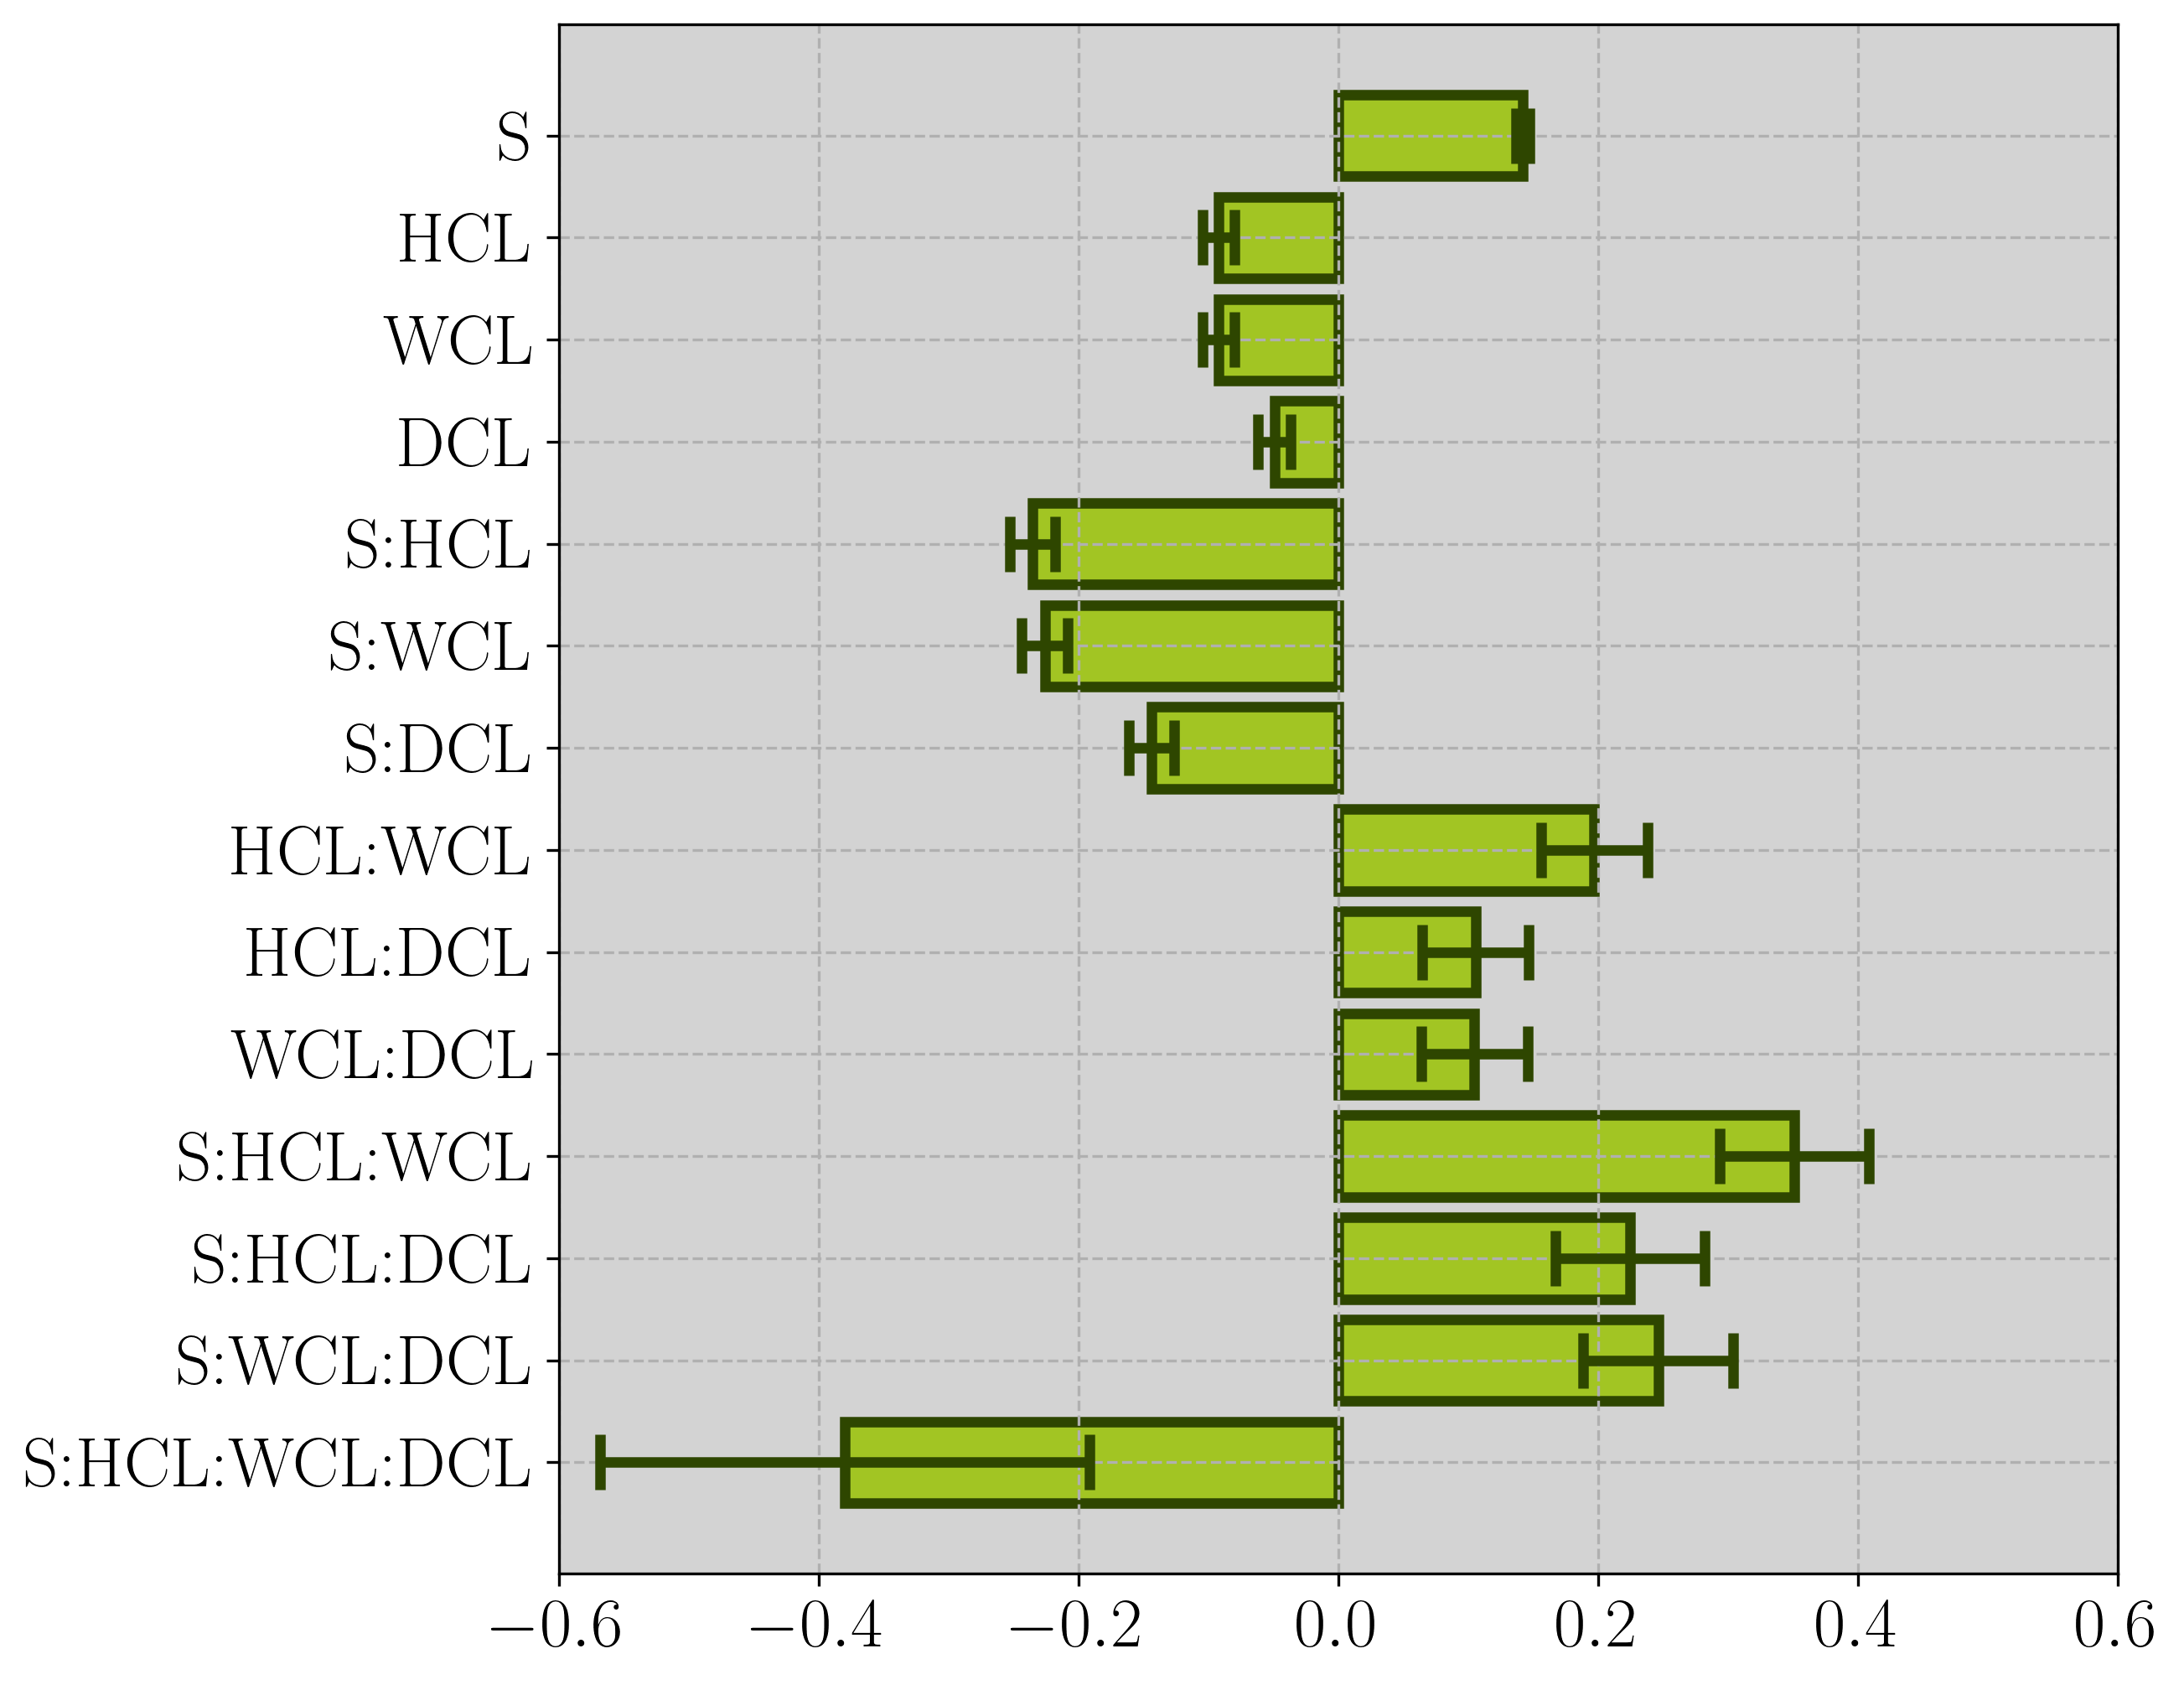
\includegraphics[width=\linewidth]{figs/SIC_Factors.png}
	\caption{Significant factors from $S_{IC}$ regression}
	\label{fig:sic_factors}
\end{figure}

\begin{table}[H]
	\centering
	\caption{Summary for $S_{IC}$ Regression}\label{tab:summary_sic}
	\begin{tabular}{|C{\linewidth/4}|C{\linewidth/4}|C{\linewidth/4}|C{\linewidth/4}|}
		\hline R & R-Squared & Adjusted R-Squared & Std. Error \\
		\hline 0.974 & 0.948 & 0.944 & 0.000 \\
		\hline
	\end{tabular}
\end{table}

\begin{table}[H]
	\centering
	\caption{ANOVA for $S_{IC}$ Regression}\label{tab:anova_sic}
	\begin{tabular}{|C{\linewidth/4}|C{\linewidth/4}|C{\linewidth/4}|C{\linewidth/4}|}
		\hline Category & Sum of Squares & DOF & Mean Squares \\
		\hline Model & 0.287 & 15 & 0.019 \\
		\hline Error & 0.016 & 234 & 0.000 \\
		\hline Total & 0.303 & 249 & 0.001 \\
		\hline  \multicolumn{2}{|c|}{$F$} &  \multicolumn{2}{c|}{$P(>F)$}  \\
		\hline  \multicolumn{2}{|c|}{283.015} &  \multicolumn{2}{c|}{0.000}  \\
		\hline
	\end{tabular}
\end{table}

\begin{table}[H]
	\centering
	\caption{Significant Factors from $S_{IC}$ Regression}\label{tab:factors_sic}
	\begin{tabular}{|C{\linewidth*1/3}|C{\linewidth*2/9}|C{\linewidth*2/9}|C{\linewidth*2/9}|}
		\hline Coefficient & Value & t-value & p-value \\
		\hline {\small Intercept } & 0.043 & 11.322 & 0.000 \\
		\hline {\small S } & 0.142 & 26.289 & 0.000 \\
		\hline {\small HCL } & -0.092 & -7.389 & 0.000 \\
		\hline {\small WCL } & -0.092 & -7.376 & 0.000 \\
		\hline {\small DCL } & -0.049 & -3.931 & 0.000 \\
		\hline {\small S:HCL } & -0.235 & -13.339 & 0.000 \\
		\hline {\small S:WCL } & -0.226 & -12.796 & 0.000 \\
		\hline {\small S:DCL } & -0.144 & -8.151 & 0.000 \\
		\hline {\small HCL:WCL } & 0.197 & 4.840 & 0.000 \\
		\hline {\small HCL:DCL } & 0.106 & 2.595 & 0.010 \\
		\hline {\small WCL:DCL } & 0.105 & 2.575 & 0.011 \\
		\hline {\small S:HCL:WCL } & 0.351 & 6.092 & 0.000 \\
		\hline {\small S:HCL:DCL } & 0.225 & 3.900 & 0.000 \\
		\hline {\small S:WCL:DCL } & 0.246 & 4.274 & 0.000 \\
		\hline {\small S:HCL:WCL:DCL } & -0.380 & -2.018 & 0.045 \\
		\hline
	\end{tabular}
\end{table}

All regression terms except HCL:WCL:DCL (interaction between home, work, and destination charger availability) were significant at 95\% confidence. Regression terms indicate that increasing charger usability likelihood results in a reduction in inconvenience and that home and work charging are more important than destination charging in achieving this. These takeaways are intuitive and in line with the findings in \cite{rabinowitz_IEEE_Access_2023}. S and S-interaction terms indicate that cost-of-uncertainty is substantial and statistically significant, proving the hypothesis of this study. All else being equal, the cost-of-uncertainty term (S) is responsible for 14\% of experienced inconvenience. Additionally, S interaction terms are additive meaning that the benefits of more charging availability and the costs of less charging availability are amplified by the effects of certainty or uncertainty.

Focusing on cost-of-uncertainty, Figure \ref{fig:sic_diff_factors} shows the significant factors resulting from regressing cost-of-uncertainty upon \gls{hcl}, \gls{wcl}, and \gls{dcl} (regression details provided in Tables \ref{tab:summary_sic_d}, \ref{tab:anova_sic_d}, and \ref{tab:factors_sic_d}).

\begin{table}[H]
	\centering
	\caption{Summary for $S_{IC}$ Difference Regression}\label{tab:summary_sic_d}
	\begin{tabular}{|C{\linewidth/4}|C{\linewidth/4}|C{\linewidth/4}|C{\linewidth/4}|}
		\hline R & R-Squared & Adjusted R-Squared & Std. Error \\
		\hline 0.924 & 0.853 & 0.843 & 0.000 \\
		\hline
	\end{tabular}
\end{table}

\begin{table}[H]
	\centering
	\caption{ANOVA for $S_{IC}$ Difference Regression}\label{tab:anova_sic_d}
	\begin{tabular}{|C{\linewidth/4}|C{\linewidth/4}|C{\linewidth/4}|C{\linewidth/4}|}
		\hline Category & Sum of Squares & DOF & Mean Squares \\
		\hline Model & 0.120 & 7 & 0.017 \\
		\hline Error & 0.030 & 117 & 0.000 \\
		\hline Total & 0.207 & 124 & 0.002 \\
		\hline  \multicolumn{2}{|c|}{$F$} &  \multicolumn{2}{c|}{$P(>F)$}  \\
		\hline  \multicolumn{2}{|c|}{65.816} &  \multicolumn{2}{c|}{0.000}  \\
		\hline
	\end{tabular}
\end{table}

\begin{table}[H]
	\centering
	\caption{Significant Factors from $S_{IC}$ Difference Regression}\label{tab:factors_sic_d}
	\begin{tabular}{|C{\linewidth*1/3}|C{\linewidth*2/9}|C{\linewidth*2/9}|C{\linewidth*2/9}|}
		\hline Coefficient & Value & t-value & p-value \\
		\hline {\small Intercept } & 0.142 & 26.709 & 0.000 \\
		\hline {\small HCL } & -0.235 & -13.552 & 0.000 \\
		\hline {\small WCL } & -0.226 & -13.001 & 0.000 \\
		\hline {\small DCL } & -0.144 & -8.281 & 0.000 \\
		\hline {\small HCL:WCL } & 0.351 & 6.190 & 0.000 \\
		\hline {\small HCL:DCL } & 0.225 & 3.963 & 0.000 \\
		\hline {\small WCL:DCL } & 0.246 & 4.342 & 0.000 \\
		\hline {\small HCL:WCL:DCL } & -0.380 & -2.050 & 0.043 \\
		\hline
	\end{tabular}
\end{table}

\begin{figure}[H]
	\centering
	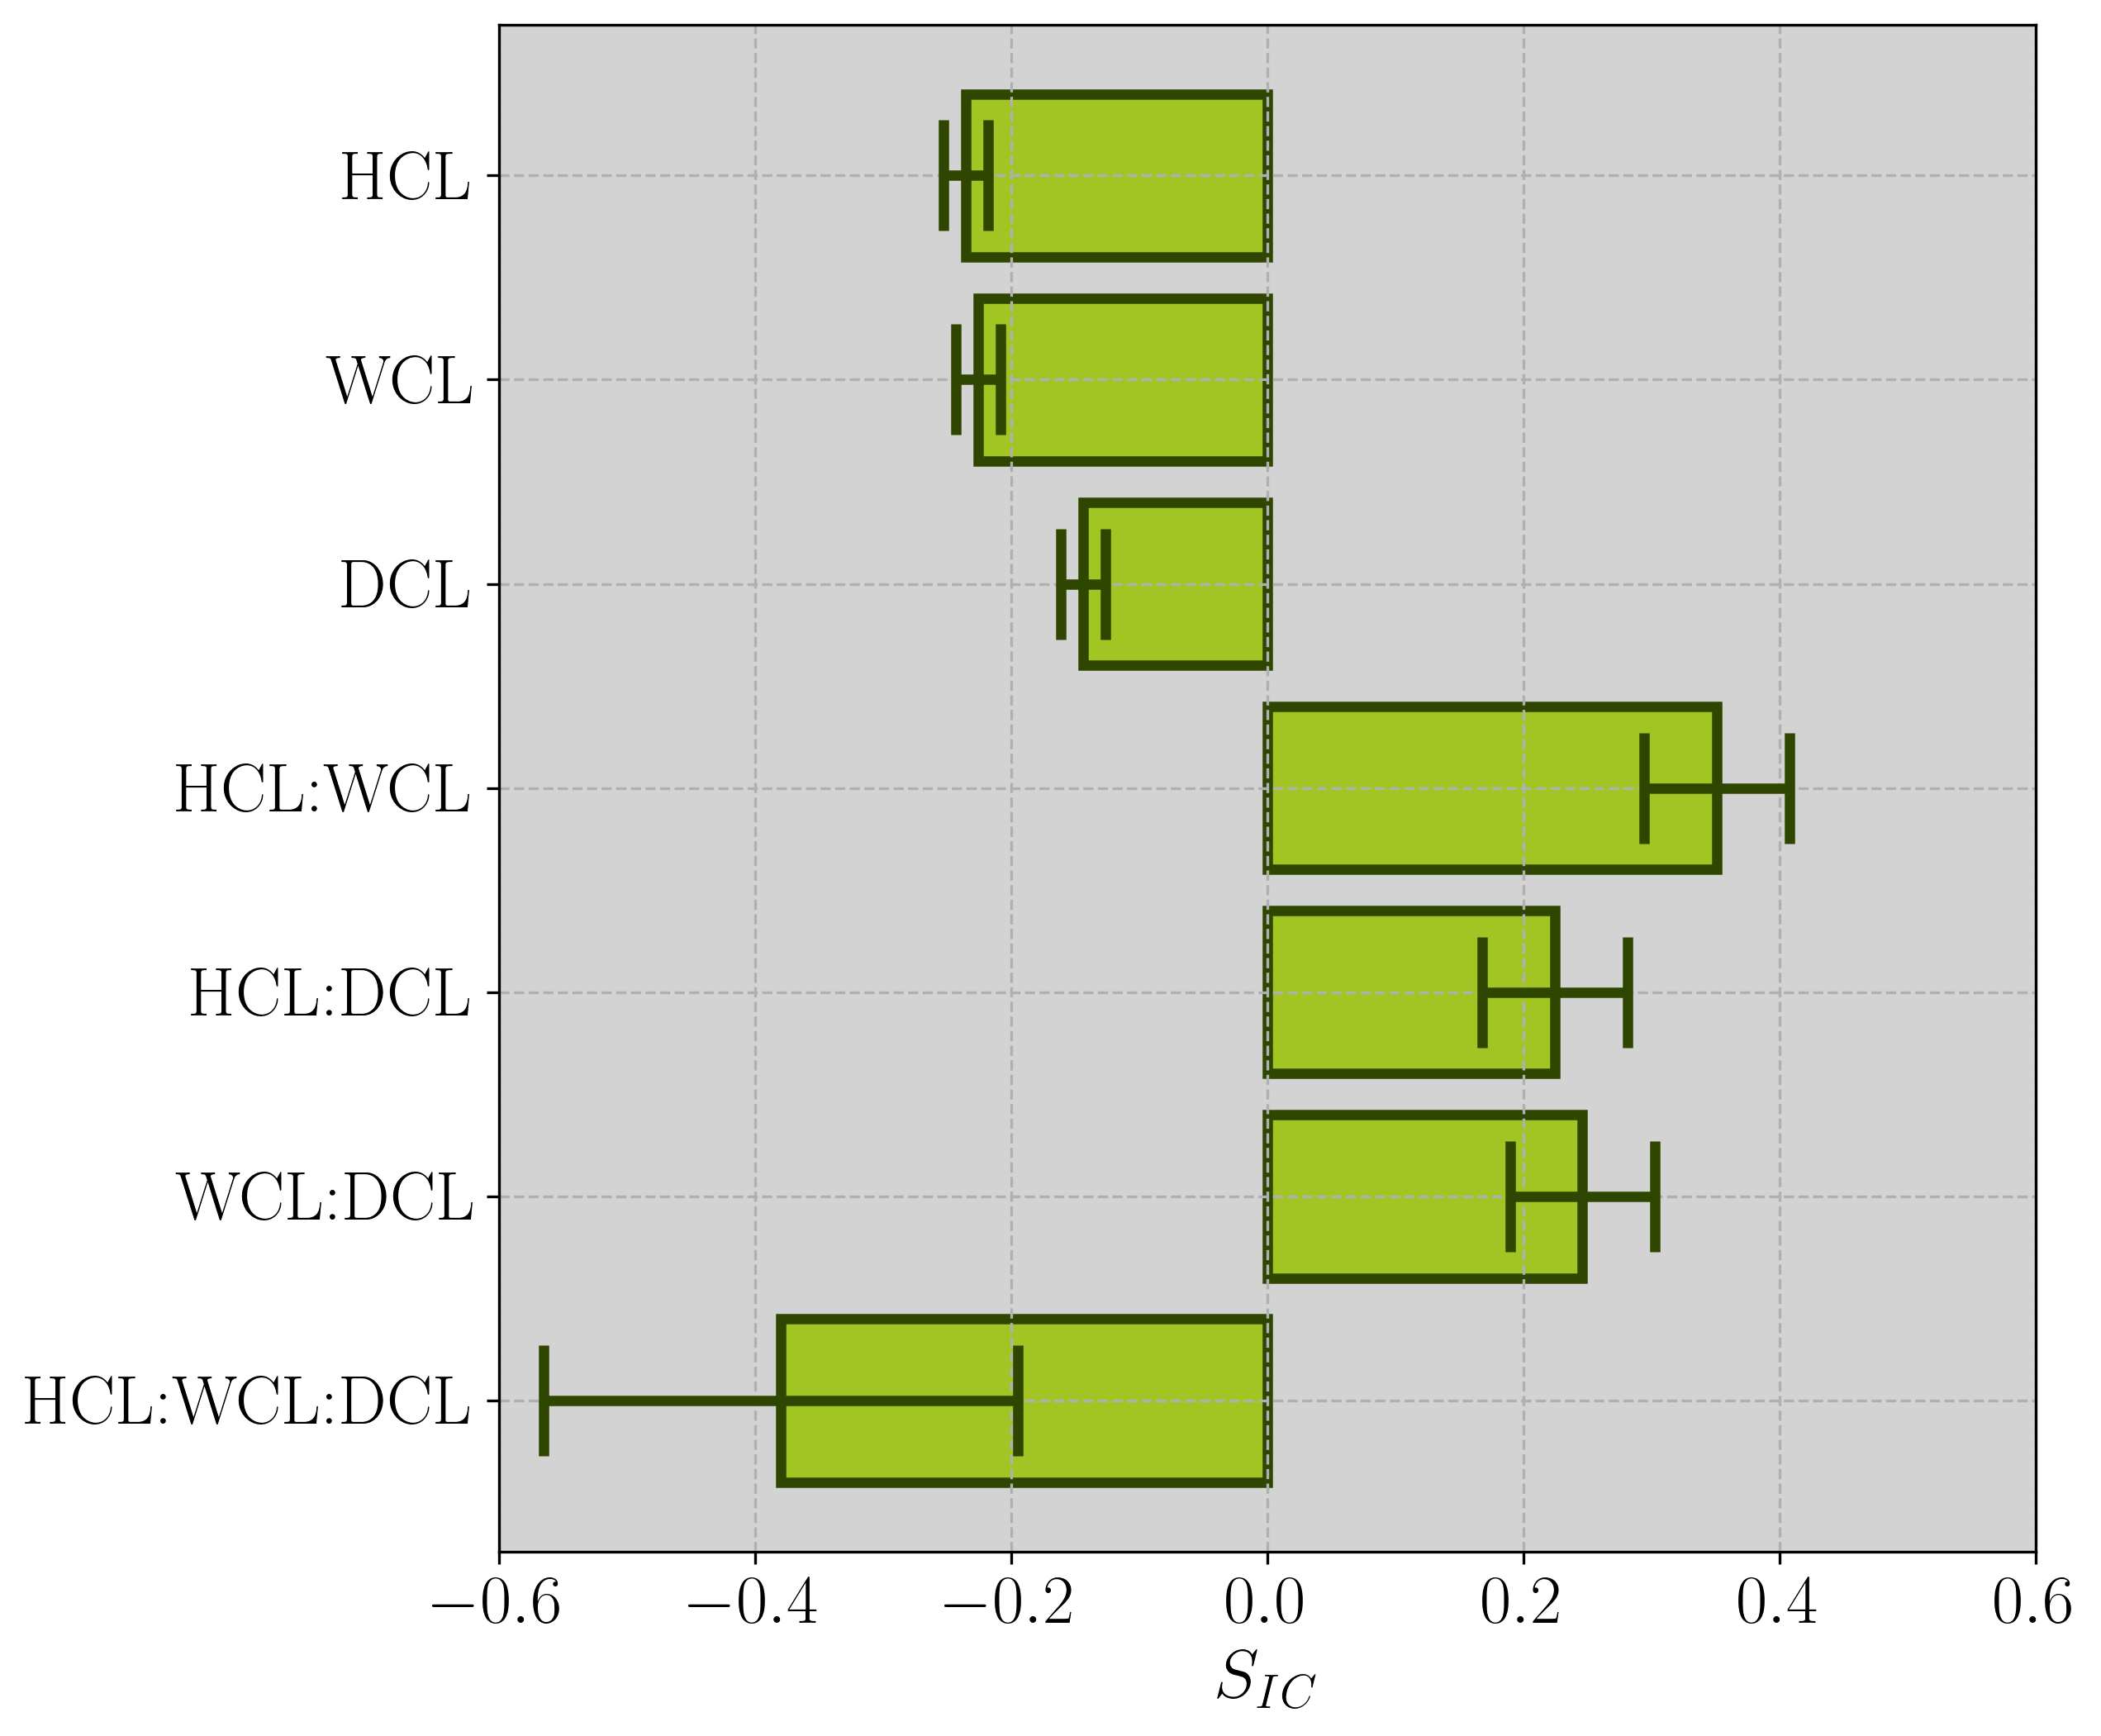
\includegraphics[width=\linewidth]{figs/SIC_Diff_Factors.png}
	\caption{Significant factors from cost-of-uncertainty regression}
	\label{fig:sic_diff_factors}
\end{figure}

\gls{hcl}, \gls{wcl}, and \gls{dcl} and all interaction terms are significant in determining cost-of-uncertainty. Increasingly reliable access to chargers at home, work, and other destinations contribute to lowering cost-of-uncertainty with home and work having more impact. The positive first order interaction terms indicate a non-additive relationship wherein \gls{bev} users with high levels of access at one location type benefit less from increasing access at others.

\section{Discussion}\label{sec:discussion}

Based on the experimental results presented in this study one can confidently accept the hypothesis that there is a non-negligible cost-of-uncertainty associated with unreliable dwell charging. The situation which inspired this study is that of multi-unit dwelling residents where the building provides some \gls{evse} but fewer charge points than parking spaces. If such individuals work away from home then they may experience similar situations at work and all will experience similar situations at public locations such as retail centers. The cost of installing and operating chargers is considerable, especially for chargers in close proximity, due to the probable need for grid enhancement \cite{Gamage_2023}. Because \gls{evse} only generates revenue while in use it is economically infeasible to maintain a saturation of chargers wherein everyone can charge whenever desired whether in public or private spaces. It follows that \gls{evse} will not always be available when desired unless the \gls{bev} user has exclusive use of \gls{evse} as is the case for residents of single family homes. The lack of guaranteed, or even likely, charger availability will result in users being more opportunistic in selecting charge events and more conservative in maintaining \gls{soc} leading to more inconvenient charge events. As a result, charging inconvenience for multi-unit dwelling residents can be expected to scale at a rate in excess of the ratio of \glspl{ev} to charge points in their buildings.

As recently as 2021 89\% of respondents to a survey conducted by NREL who were owners of single-unit-detached dwellings claimed possible access to home charging while this number was only 29\% for renters in high-capacity \glspl{mud}. The latter number does not account for the number of \glspl{bev} per charger. In the past it might be safe to assume that the number of electric vehicles in a given \gls{mud} will be fairly small. Since 2021, \gls{ev} sales have risen rapidly in the US and globally \cite{KBB_2023,EVVolumes_2023} and such assumptions will break down shortly if they have not already. It is, thus, imperative that \gls{evse} subsidy programs begin to place high emphasis on \glspl{mud} and workplaces. While not equivalent to adding more chargers certain policies can mitigate the cost-of-uncertainty associated with shared charging resources. These policies include pricing schemes which discourage over-long charge events for public spaces \cite{Nicholas_2013} and scheduled charging sessions for private spaces. Such policies can help to maintain rational behavior and efficient allocation of shared charging resources allowing for fewer resources to be sufficient for a larger user base.

\section{Conclusions}\label{sec:concusions}

Continued \gls{bev} market penetration depends on a growing stream of new adopters and low discontinuance rates among current adopters. To a point, new adopters can be enticed with incentives but, ultimately, \glspl{bev} must win out on the strength of their fundamentals. As \gls{bev} purchase prices come down, \glspl{bev} become strong options for more and more of the market. However, there is a distinct and enduring difference in the value proposition for two groups of vehicle users, those with access to exclusive home AC level 2 charging and those without. The difference manifests as both a financial and time cost as the latter group are forced to select costly and inconvenient charging events more often than the former. Addressing this inequity requires understanding how reliance on shared community \gls{evse} effects user behavior. With insufficient resources and governance users of shared resources will see limited benefits. In this paper, a quantitative method is provided which extends on the authors' previous charging inconvenience work to account for the cost-of-uncertainty associated with uncertain \gls{evse} availability. Results of a designed computational experiment using real driving data show a statistically significant and substantial cost-of-uncertainty for \gls{bev} users reliant on public and shared \gls{evse}. The experience of said users may be improved via investments in additional \gls{evse} and by the implementation of governance policies such as financial disincentives for prolonged charge events and scheduled access. The relationship between \gls{evse} expansion and reduction of uncertainty is additive and future \gls{evse} subsidy programs which include governance requirements may be more successful than those which do not.

\bibliographystyle{ieeetr}
\bibliography{sources}
\end{document}
